% vim: set spell spelllang=en_gb

\chapter{Introduction}


\guidance{%
  The Introduction should explain the \textbf{principal motivation} for the
  project.  \textbf{Show how the work fits into} the broad area of surrounding
  Computer Science and \textbf{give a brief survey} of previous related work.
  It should \textbf{generally be unnecessary to quote at length} from technical
  papers or textbooks. If a simple bibliographic reference is insufficient,
  consign any lengthy quotation to an appendix.
}

\prechapter{%
  Coq is an interactive proof-assistant~\cite{Coq:manual}; it allows users to
  formalise mathematical theories into machine-checked proofs. Coq libraries,
  which encode mathematical theories, are difficult to understand. In this
  dissertation, I will describe a new tool I implemented for Coq users that
  aimed to (a) represent Coq libraries as Neo4j (graph) databases and (b)
  provide a library of queries with the goal of highlighting the structure and
  relationship between the representations of the proof-objects by using
  network-analysis techniques usually associated with social-networks.
}


\section{Motivation}

Coq proof-scripts are notoriously difficult to understand. Not only do these
proof-scripts encode a mathematical theory, which can be difficult to
understand in and of itself, they serve as verbose instructions on how to
create proof-term whose type matches a certain proposition, rather than a
statement of \emph{why} something is true. There are currently no tools which
help with the challenge of gaining a \emph{high-level} understanding of a large
Coq library.

The Feit-Thompson Odd Order Theorem~\cite{peterfalvi2000oot, bender1994oot}
(which has been translated into Coq~\cite{gonthier2013oot}) is an example of a
large Coq library. It is a part of larger, general trend of formalising
substantial bodies of mathematics and marks the first time that we have a new
way representing mathematics, different from the combination of formulas and
natural-language prose usually used. Such a turning point provides an
opportunity to explore the novel representations and analyses possible.

However, it is still the case that when a user approaches a large Coq library, 
they are left to understand and keep track of several aspects of the
library (such as implicit assumptions, previously defined results and the
types and conventions behind any notation) by themself. There is very little
opportunity to consider and compare different approaches for arriving at a
result (i.e.\ number of assumptions, number of steps, some notion of the
importance such as number of uses).

I obtained such an opportunity by using a query-based approach: by creating a
tool that expresses Coq library as databases, then I was able query them and
analyse them to gain insights such as those mentioned above.

\section{A Database Approach}

Mathematical theories are highly interconnected structures of definitions and
proofs. As such, relational or a document-oriented models are not adequate
representations for answering questions such as ``What depends on this lemma
and how many such things are there?'' or ``What are the components of this
definition?''.

Even a static, graph-based approach on its own is insufficient. Simply
outputting a dependency graph is ineffective for all but the smallest of
libraries. Figure~\ref{fig:static} shows one such dependency graph for a
medium-sized Coq library.

\begin{figure}[tp]

  \centering
  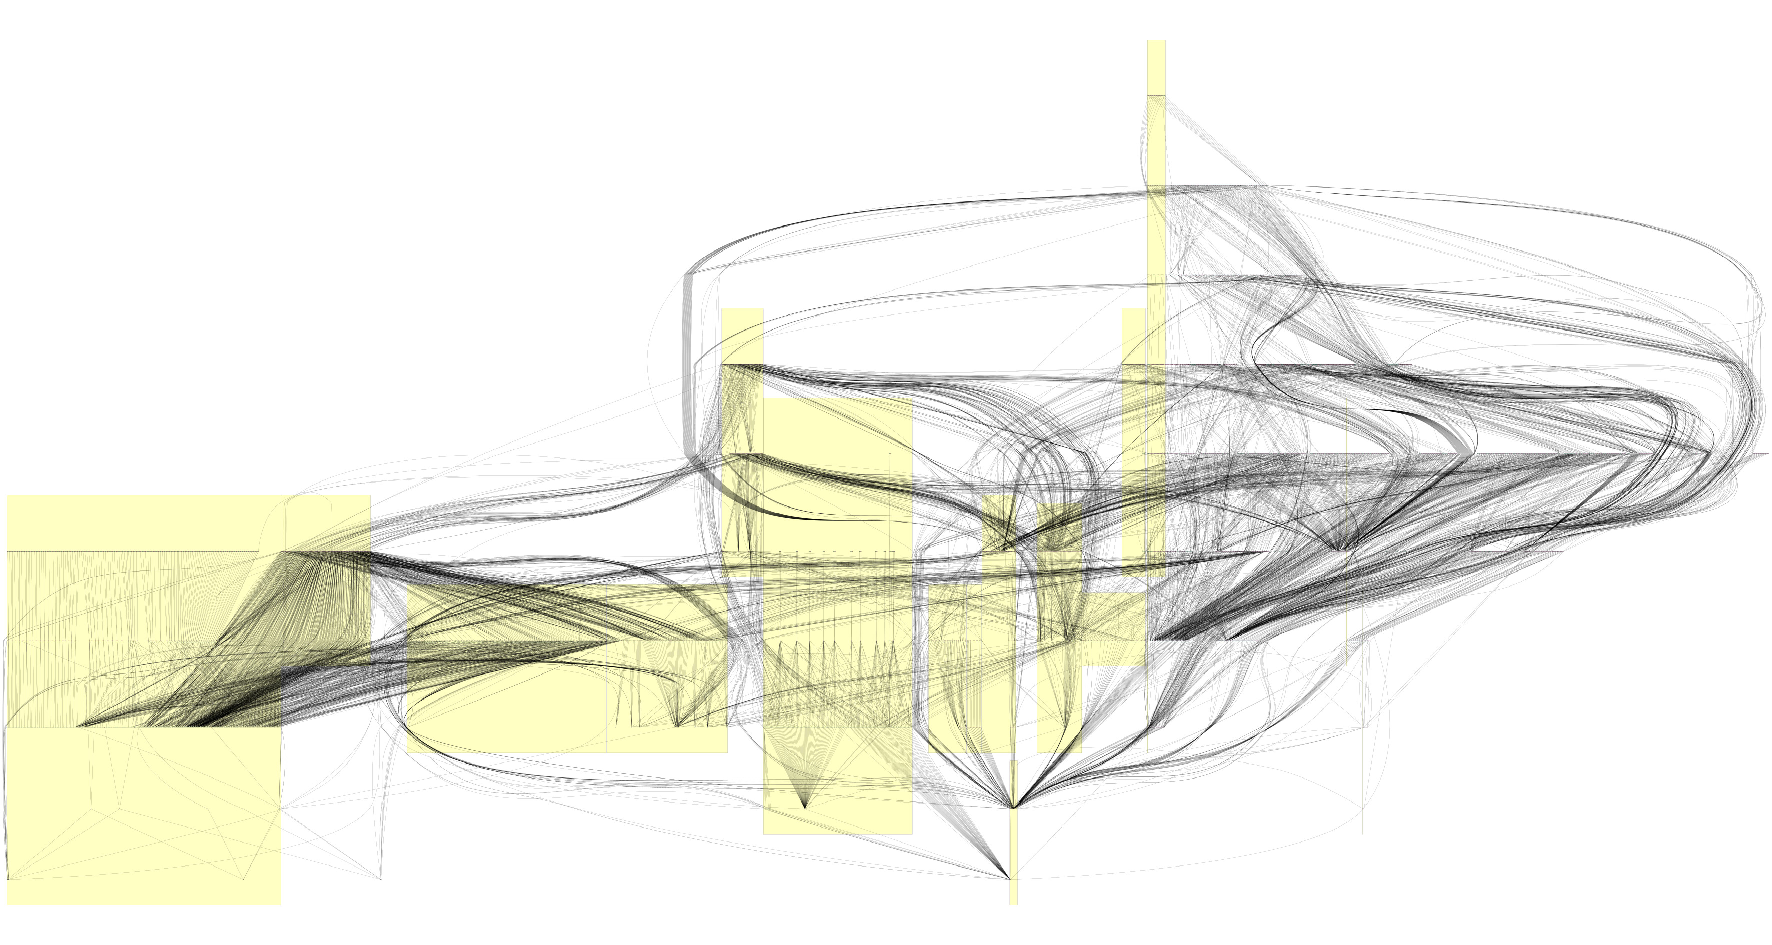
\includegraphics[width=\textwidth, page=1]{img/static-CAS-small.pdf}
  \caption{Static graph of
    \href{https://github.com/Timothy-G-Griffin/CAS}{CAS} Coq library. For all
    but the smallest of libraries, simply outputting a dependency graph is an
    ineffective way of understanding them.}\label{fig:static}

\end{figure}

\emph{Graph databases} have been developed to deal with highly connected data
sets and path-oriented queries. That is, graph databases are optimised for
computing transitive-closure and related queries, which pose a huge challenge
for traditional, relational databases. Due to the emergence of massive data
sets thanks to large-scale social and advertising networks, new techniques for
representing and analysing such data have been developed.

\newpage
For this project, I used the Neo4j~\cite{neo4j} graph database system (and its
expressive query language \emph{Cypher}) to create a tool for Coq users which
applies such network-analysis techniques to Coq libraries to aid understanding
them.

\section{Aims of the Project}\label{intro:aims}

In this project, I aimed to write a tool for Coq users that:

\begin{itemize}
\item represents Coq libraries as Neo4j graph databases, which consists of
  \begin{itemize}
  \item exploring and choosing the correct model
  \item converting and extending existing code to output CSVs
  \item writing new programs to extract extra information \\
      (omitted from other, existing tools)
  \item writing new programs to automate database creation.
  \end{itemize}

\item provides a library of Neo4j queries, intended
  \begin{itemize}
  \item to highlight the structure of and relationship between proof-objects
  \item to provide several network-analysis techniques.
  \end{itemize}
\end{itemize}

Note that the aims centre around the \emph{mechanics and details} of creating a
model for Coq proof-objects and applying network analysis techniques to it and
\emph{not creating a polished, user-friendly product}. Since \emph{usability was
not a \emph{primary} focus of this project}, I did not conduct a user-study whilst
evaluating this tool.

\newpage

\section{Summary}

First, I explained why Coq libraries difficult to understand. Then, I said
that the trend of formalising large bodies of mathematics such as the
Feit-Thompson Odd Order Theorem~\cite{peterfalvi2000oot, bender1994oot}
presents an opportunity to develop new representations and analyses of
mathematical theories. After that, I outlined why databases, specifically
graph databases, were a promising approach to this new opportunity. Finally, I
listed the aims of this project.
